%%%%%%%%%%%%%%%%%%%%% chapter.tex %%%%%%%%%%%%%%%%%%%%%%%%%%%%%%%%%
%
% sample chapter
%
% Use this file as a template for your own input.
%
%%%%%%%%%%%%%%%%%%%%%%%% Springer-Verlag %%%%%%%%%%%%%%%%%%%%%%%%%%
%\motto{Use the template \emph{chapter.tex} to style the various elements of your chapter content.}

\chapter{Rosetta Code Tasks starting with F}

\section*{Factorial}

The \textbf{Factorial Function} of a positive integer, \emph{n}, is
defined as the product of the sequence \emph{n}, \emph{n}-1, \emph{n}-2,
\ldots{}1 and the factorial of zero, 0, is
\href{http://en.wikipedia.org/wiki/Factorial\#Definition}{defined} as
being 1.

Write a function to return the factorial of a number. Solutions can be
iterative or recursive. Support for trapping negative n errors is
optional.

\begin{wideverbatim}

(de fact (N)
   (if (=0 N)
      1
      (* N (fact (dec N))) ) )

or

(de fact (N)
   (apply * (range 1 N)) )

\end{wideverbatim}

\pagebreak{}
\section*{Factors of a Mersenne number}

A Mersenne number is a number in the form of 2\textsuperscript{P}-1.
If P is prime, the Mersenne number may be a Mersenne prime (if P is
not prime, the Mersenne number is also not prime). In the search for
Mersenne prime numbers it is advantageous to eliminate exponents by
finding a small factor before starting a, potentially lengthy,
\emph{Lucas-Lehmer test}. There are very efficient algorithms for
determining if a number divides 2\textsuperscript{P}-1 (or
equivalently, if 2\textsuperscript{P} mod (the number) = 1). Some
languages already have built-in implementations of this
exponent-and-mod operation (called \emph{modPow} or similar). The
following is how to implement this \emph{modPow} yourself:

For example, let's compute 2\textsuperscript{23} mod 47. Convert the
exponent 23 to binary, you get 10111. Starting with \texttt{square} = 1,
repeatedly square it. Remove the top bit of the exponent, and if it's 1
multiply \texttt{square} by the base of the exponentiation (2), then
compute \texttt{square} modulo 47. Use the result of the modulo from the
last step as the initial value of \texttt{square} in the next step:

\begin{verbatim}
                 Remove   Optional   
   square        top bit  multiply by 2  mod 47
   ------------  -------  -------------  ------
   1*1 = 1       1  0111  1*2 = 2           2
   2*2 = 4       0   111     no             4
   4*4 = 16      1    11  16*2 = 32        32
   32*32 = 1024  1     1  1024*2 = 2048    27
   27*27 = 729   1        729*2 = 1458      1
\end{verbatim}

Since 2\textsuperscript{23} mod 47 = 1, 47 is a factor of
2\textsuperscript{P}-1. (To see this, subtract 1 from both sides:
2\textsuperscript{23}-1 = 0 mod 47.) Since we've shown that 47 is a
factor, 2\textsuperscript{23}-1 is not prime. Further properties of
Mersenne numbers allow us to refine the process even more. Any factor
q of 2\textsuperscript{P}-1 must be of the form 2kP+1, k being a
positive integer or zero. Furthermore, q must be 1 or 7 mod 8. Finally
any potential factor q must be \emph{prime}. As in other trial
division algorithms, the algorithm stops when 2kP+1 \textgreater{}
sqrt(N).

These primality tests only work on Mersenne numbers where P is prime.
For example, M\textsubscript{4}=15 yields no factors using these
techniques, but factors into 3 and 5, neither of which fit 2kP+1.

\textbf{Task:} Using the above method find a factor of
2\textsuperscript{929}-1 (aka M929)


\begin{wideverbatim}

(de **Mod (X Y N)
   (let M 1
      (loop
         (when (bit? 1 Y)
            (setq M (\% (* M X) N)) )
         (T (=0 (setq Y (>> 1 Y)))
            M )
         (setq X (\% (* X X) N)) ) ) )

(de prime? (N)
   (or
      (= N 2)
      (and
         (> N 1)
         (bit? 1 N)
         (for (D 3  T  (+ D 2))
            (T (> D (sqrt N)) T)
            (T (=0 (\% N D)) NIL) ) ) ) )

(de mFactor (P)
   (let (Lim (sqrt (dec (** 2 P)))  K 0  Q)
      (loop
         (setq Q (inc (* 2 (inc 'K) P)))
         (T (>= Q Lim) NIL)
         (T
            (and
               (member (\% Q 8) (1 7))
               (prime? Q)
               (= 1 (**Mod 2 P Q)) )
            Q ) ) ) )

\end{wideverbatim}

\begin{wideverbatim}


Output:

: (for P (2 3 4 5 7 11 13 17 19 23 29 31 37 41 43 47 53 929)
   (prinl
      "M" P " = 2**" P "-1 is "
      (cond
         ((not (prime? P)) "not prime")
         ((mFactor P) (pack "composite with factor " @))
         (T "prime") ) ) )
M2 = 2**2-1 is prime
M3 = 2**3-1 is prime
M4 = 2**4-1 is not prime
M5 = 2**5-1 is prime
M7 = 2**7-1 is prime
M11 = 2**11-1 is composite with factor 23
M13 = 2**13-1 is prime
M17 = 2**17-1 is prime
M19 = 2**19-1 is prime
M23 = 2**23-1 is composite with factor 47
M29 = 2**29-1 is composite with factor 233
M31 = 2**31-1 is prime
M37 = 2**37-1 is composite with factor 223
M41 = 2**41-1 is composite with factor 13367
M43 = 2**43-1 is composite with factor 431
M47 = 2**47-1 is composite with factor 2351
M53 = 2**53-1 is composite with factor 6361
M929 = 2**929-1 is composite with factor 13007

\end{wideverbatim}

\pagebreak{}
\section*{Factors of an integer}

\textbf{Basic Data Operation}\\ This is a basic data operation. It
represents a fundamental action on a basic data type.

You may see other such operations in the \emph{Basic Data Operations}
category, or:

\textbf{Integer Operations} \\
\emph{Arithmetic} \textbar{} \emph{Comparison}

\textbf{Boolean Operations} \\ \emph{Bitwise} \textbar{}
\emph{Logical}

\textbf{String Operations} \\
\emph{Concatenation} \textbar{} \emph{Interpolation} \textbar{}
\emph{Matching}

\textbf{Memory Operations} \\
\emph{Pointers \& references} \textbar{} \emph{Addresses}

Compute the \href{http://en.wikipedia.org/wiki/Divisor}{factors} of a
positive integer. These factors are the positive integers by which the
number being factored can be divided to yield a positive integer result
(though the concepts function correctly for zero and negative integers,
the set of factors of zero is has countably infinite members, and the
factors of negative integers can be obtained from the factors of related
positive numbers without difficulty; this task does not require handling
of either of these cases). Note that even prime numbers will have at
least two factors; `1' and themselves.

See also:

\begin{itemize}
\item
  \emph{Prime decomposition}
\end{itemize}


\begin{wideverbatim}

(de factors (N)
   (filter
      '((D) (=0 (% N D)))
      (range 1 N) ) )
\end{wideverbatim}

\pagebreak{}
\section*{Fast Fourier transform}

The purpose of this task is to calculate the FFT (Fast Fourier
Transform) of an input sequence. The most general case allows for
complex numbers at the input and results in a sequence of equal length,
again of complex numbers. If you need to restrict yourself to real
numbers the output should be the magnitude (i.e. sqrt(re²+im²)) of the
complex result. The classic version is the recursive Cooley--Tukey FFT.
\href{http://en.wikipedia.org/wiki/Cooley--Tukey\_FFT\_algorithm}{Wikipedia}
has pseudocode for that. Further optimizations are possible but not
required.


\begin{wideverbatim}

{{works with|PicoLisp|3.1.0.3}}

# apt-get install libfftw3-dev

(scl 4)

(de FFTW_FORWARD . -1)
(de FFTW_ESTIMATE . 64)

(de fft (Lst)
   (let
      (Len (length Lst)
         In (native "libfftw3.so" "fftw_malloc" 'N (* Len 16))
         Out (native "libfftw3.so" "fftw_malloc" 'N (* Len 16))
         P (native "libfftw3.so" "fftw_plan_dft_1d" 'N
            Len In Out FFTW_FORWARD FFTW_ESTIMATE ) )
      (struct In NIL (cons 1.0 (apply append Lst)))
      (native "libfftw3.so" "fftw_execute" NIL P)
      (prog1 (struct Out (make (do Len (link (1.0 . 2)))))
         (native "libfftw3.so" "fftw_destroy_plan" NIL P)
         (native "libfftw3.so" "fftw_free" NIL Out)
         (native "libfftw3.so" "fftw_free" NIL In) ) ) )

Test:

(for R (fft '((1.0 0) (1.0 0) (1.0 0) (1.0 0) (0 0) (0 0) (0 0) (0 0)))
   (tab (6 8)
      (round (car R))
      (round (cadr R)) ) )

Output:

 4.000   0.000
 1.000  -2.414
 0.000   0.000
 1.000  -0.414
 0.000   0.000
 1.000   0.414
 0.000   0.000
 1.000   2.414

\end{wideverbatim}

\pagebreak{}
\section*{Fibonacci n-step number sequences}

These number series are an expansion of the ordinary
\emph{Fibonacci sequence} where:


The \textbf{Fibonacci sequence} is a sequence F\textsubscript{n} of
natural numbers defined recursively:

\begin{verbatim}
F0 = 0
F1 = 1
Fn = Fn-1 + Fn-2, if n>1
\end{verbatim}

Write a function to generate the nth Fibonacci number. Solutions can be
iterative or recursive (though recursive solutions are generally
considered too slow and are mostly used as an exercise in recursion).

The sequence is sometimes extended into negative numbers by using a
straightforward inverse of the positive definition:

\begin{verbatim}
Fn = Fn+2 - Fn+1, if n<0
\end{verbatim}

Support for negative n in the solution is optional.

\begin{description}
\item[Cf.]
\end{description}

\begin{itemize}
\item \emph{Fibonacci n-step number sequences‎}
\end{itemize}

\begin{description}
\item[References]
\end{description}

\begin{itemize}
\item
  \href{http://en.wikipedia.org/wiki/Fibonacci\_number}{Wikipedia,
  Fibonacci number}
\item
  \href{http://en.wikipedia.org/wiki/Lucas\_number}{Wikipedia, Lucas
  number}
\item
  \href{http://mathworld.wolfram.com/FibonacciNumber.html}{MathWorld,
  Fibonacci Number}
\item
  \href{http://www.math-cs.ucmo.edu/~curtisc/articles/howardcooper/genfib4.pdf}{Some
  identities for r-Fibonacci numbers}
\item
  \href{http://oeis.org/A000045}{OEIS Fibonacci numbers}
\item
  \href{http://oeis.org/A000032}{OEIS Lucas numbers}
\end{itemize}



\begin{enumerate}
\item
  For \emph{n} = 2 we have the Fibonacci sequence; with initial values
  {[}1,1{]} and
  \begin{figure}[H]
    \centering
    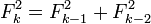
\includegraphics[scale=.6]{graphics/ea8fba6081e51a2e4f0cd0d58c3c7032.png}    
  \end{figure}
\item
  For \emph{n} = 3 we have the tribonacci sequence; with initial values
  {[}1,1,2{]} and
  \begin{figure}[H]
    \centering
     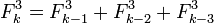
\includegraphics[scale=.6]{graphics/a96e7fe6a7eb7371ab85f6a135b84056.png}    
  \end{figure}
\item
  For \emph{n} = 4 we have the tetranacci sequence; with initial values
  {[}1,1,2,4{]} and
  \begin{figure}[H]
    \centering
    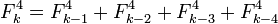
\includegraphics[scale=.6]{graphics/ea2b3ddffa2a578dbe5d923abd914aa5.png}
  \end{figure}

\ldots{}    

\item
  For general \emph{n} \textgreater{} 2 we have the Fibonacci
  \emph{n}-step sequence -
  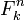
\includegraphics[scale=.6]{graphics/f6e22469b4396d8fa34e202e5c716abc.png};
  with initial values of the first \emph{n} values of the (\emph{n} −
  1)'th Fibonacci \emph{n}-step sequence
  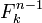
\includegraphics[scale=.6]{graphics/79293ba1053dbc3f23c579b2e8141034.png};
  and \emph{k}'th value of this \emph{n}'th sequence being

  \begin{figure}[H]
    \centering
     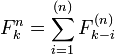
\includegraphics[scale=.6]{graphics/c53daded435e185afefbac417fef75e7.png}    
  \end{figure}
\end{enumerate}

For small values of \emph{n},
\href{http://en.wikipedia.org/wiki/Number\_prefix\#Greek\_series}{Greek
numeric prefixes} are sometimes used to individually name each series.

\ctable[caption = { Fibonacci \emph{n}-step sequences },
pos = H, center, botcap]{lll}
{% notes
}
{% rows
\FL
\emph{n} & Series name & Values
\ML
2 & fibonacci & 1 1 2 3 5 8 13 21 34 55 89 144 233 377 610 \ldots{}
\\\noalign{\medskip}
3 & tribonacci & 1 1 2 4 7 13 24 44 81 149 274 504 927 1705 3136
\ldots{}
\\\noalign{\medskip}
4 & tetranacci & 1 1 2 4 8 15 29 56 108 208 401 773 1490 2872 5536
\ldots{}
\\\noalign{\medskip}
5 & pentanacci & 1 1 2 4 8 16 31 61 120 236 464 912 1793 3525 6930
\ldots{}
\\\noalign{\medskip}
6 & hexanacci & 1 1 2 4 8 16 32 63 125 248 492 976 1936 3840 7617
\ldots{}
\\\noalign{\medskip}
7 & heptanacci & 1 1 2 4 8 16 32 64 127 253 504 1004 2000 3984 7936
\ldots{}
\\\noalign{\medskip}
8 & octonacci & 1 1 2 4 8 16 32 64 128 255 509 1016 2028 4048 8080
\ldots{}
\\\noalign{\medskip}
9 & nonanacci & 1 1 2 4 8 16 32 64 128 256 511 1021 2040 4076 8144
\ldots{}
\\\noalign{\medskip}
10 & decanacci & 1 1 2 4 8 16 32 64 128 256 512 1023 2045 4088 8172
\ldots{}
\LL
}

Allied sequences can be generated where the initial values are changed:

\textbf{The \href{http://en.wikipedia.org/wiki/Lucas\_number}{Lucas
series}} sums the two preceeding values like the fibonacci series for
\emph{n} = 2 but uses {[}2,1{]} as its initial values.

\pagebreak{}
\begin{description}
\item[The task is to]
\end{description}

\begin{enumerate}
\item
  Write a function to generate Fibonacci \emph{n}-step number sequences
  given its initial values and assuming the number of initial values
  determines how many previous values are summed to make the next number
  of the series.
\item
  Use this to print and show here at least the first ten members of the
  Fibo/tribo/tetra-nacci and Lucas sequences.
\end{enumerate}

\begin{description}
\item[Cf.]
\end{description}

\begin{itemize}
\item \emph{Fibonacci sequence}
\item
  \href{http://mathworld.wolfram.com/Fibonaccin-StepNumber.html}{Wolfram
  Mathworld}
\item \emph{Hofstadter Q sequence‎}
\end{itemize}


\begin{wideverbatim}

(de nacci (Init Cnt)
   (let N (length Init)
      (make
         (made Init)
         (do (- Cnt N)
            (link (apply + (tail N (made)))) ) ) ) )

Test:
# Fibonacci
: (nacci (1 1) 10)
-> (1 1 2 3 5 8 13 21 34 55)

# Tribonacci
: (nacci (1 1 2) 10)
-> (1 1 2 4 7 13 24 44 81 149)

# Tetranacci
: (nacci (1 1 2 4) 10)
-> (1 1 2 4 8 15 29 56 108 208)

# Lucas
: (nacci (2 1) 10)
-> (2 1 3 4 7 11 18 29 47 76)

# Decanacci
: (nacci (1 1 2 4 8 16 32 64 128 256) 15)
-> (1 1 2 4 8 16 32 64 128 256 512 1023 2045 4088 8172)

\end{wideverbatim}

\pagebreak{}
\section*{Fibonacci sequence}

The \textbf{Fibonacci sequence} is a sequence F\textsubscript{n} of
natural numbers defined recursively:

\begin{verbatim}
F0 = 0
F1 = 1
Fn = Fn-1 + Fn-2, if n>1
\end{verbatim}

Write a function to generate the nth Fibonacci number. Solutions can be
iterative or recursive (though recursive solutions are generally
considered too slow and are mostly used as an exercise in recursion).

The sequence is sometimes extended into negative numbers by using a
straightforward inverse of the positive definition:

\begin{verbatim}
Fn = Fn+2 - Fn+1, if n<0
\end{verbatim}

Support for negative n in the solution is optional.

\begin{description}
\item[Cf.]
\end{description}

\begin{itemize}
\item \emph{Fibonacci n-step number sequences‎}
\end{itemize}

\begin{description}
\item[References]
\end{description}

\begin{itemize}
\item
  \href{http://en.wikipedia.org/wiki/Fibonacci\_number}{Wikipedia,
  Fibonacci number}
\item
  \href{http://en.wikipedia.org/wiki/Lucas\_number}{Wikipedia, Lucas
  number}
\item
  \href{http://mathworld.wolfram.com/FibonacciNumber.html}{MathWorld,
  Fibonacci Number}
\item
  \href{http://www.math-cs.ucmo.edu/~curtisc/articles/howardcooper/genfib4.pdf}{Some
  identities for r-Fibonacci numbers}
\item
  \href{http://oeis.org/A000045}{OEIS Fibonacci numbers}
\item
  \href{http://oeis.org/A000032}{OEIS Lucas numbers}
\end{itemize}


\begin{wideverbatim}

Recursive

(de fibo (N)
   (if (> 2 N)
      1
      (+ (fibo (dec N)) (fibo (- N 2))) ) )

Recursive with Cache

Using a recursive version doesn't need to be slow, as the following shows:

(de fibo (N)
   (cache '(NIL) (pack (char (hash N)) N)  # Use a cache to accelerate
      (if (> 2 N)
         N
         (+ (fibo (dec N)) (fibo (- N 2))) ) ) )

(bench (fibo 1000))

Output:

0.012 sec
-> 43466557686937456435688527675040625802564660517371780402481729089536555417949
05189040387984007925516929592259308032263477520968962323987332247116164299644090
6533187938298969649928516003704476137795166849228875

\end{wideverbatim}

\pagebreak{}
\section*{File IO}


\textbf{File IO} is part of \emph{Short Circuit}'s
\textbf{\href{/wiki/Category:Selection/Short\_Circuit/Console\_Program\_Basics}{Console
    Program Basics}} selection.

In this task, the job is to create a file called ``output.txt'', and
place in it the contents of the file ``input.txt'', \emph{via an
intermediate variable.} In other words, your program will demonstrate:
(1) how to read from a file into a variable, and (2) how to write a
variable's contents into a file. Oneliners that skip the intermediate
variable are of secondary interest --- operating systems have copy
commands for that.

\begin{wideverbatim}

# Using a variable

(let V (in "input.txt" (till))
   (out "output.txt" (prin V)) )

# Skipping intermediate variable

(in "input.txt"
   (out "output.txt"
      (echo) ) )

\end{wideverbatim}

\pagebreak{}
\section*{File modification time}

This task will attempt to get and set the modification time of a file.

\begin{wideverbatim}

(let File "test.file"
   (and
      (info File)
      (prinl (stamp (cadr @) (cddr @))) ) # Print date and time in UTC
   (call 'touch File) )                   # Set modification time to "now"

\end{wideverbatim}

\pagebreak{}
\section*{File size}

In this task, the job is to verify the size of a file called
``input.txt'' for a file in the current working directory and another
one in the file system root.

\begin{wideverbatim}

(println (car (info "input.txt")))
(println (car (info "/input.txt")))

\end{wideverbatim}

\pagebreak{}
\section*{Filter}

Select certain elements from an Array into a new Array in a generic way.
To demonstrate, select all even numbers from an Array.

As an option, give a second solution which filters destructively, by
modifying the original Array rather than creating a new Array.

\begin{wideverbatim}

(filter '((N) (not (bit? 1 N)))
   (1 2 3 4 5 6 7 8 9) )

Output:

-> (2 4 6 8)

\end{wideverbatim}

\pagebreak{}
\section*{Find Common Directory Path}

Create a routine that, given a set of strings representing directory
paths and a single character directory separator, will return a string
representing that part of the directory tree that is common to all the
directories.

Test your routine using the forward slash `/' character as the directory
separator and the following three strings as input paths:

\begin{verbatim}
 '/home/user1/tmp/coverage/test'
 '/home/user1/tmp/covert/operator'
 '/home/user1/tmp/coven/members'
\end{verbatim}

Note: The resultant path should be the valid directory
\texttt{'/home/user1/tmp'} and not the longest common string
\texttt{'/home/user1/tmp/cove'}.

If your language has a routine that performs this function (even if it
does not have a changeable separator character, then mention it as
part of the task)

\begin{wideverbatim}

(de commonPath (Lst Chr)
   (glue Chr
      (make
         (apply find
            (mapcar '((L) (split (chop L) Chr)) Lst)
            '(@ (or (pass <>) (nil (link (next))))) ) ) ) )

Output:

(commonPath
   (quote
      "/home/user1/tmp/coverage/test"
      "/home/user1/tmp/covert/operator"
      "/home/user1/tmp/coven/members" )
   "/" )

-> "/home/user1/tmp"

\end{wideverbatim}

\pagebreak{}
\section*{Find first and last set bit of a long integer}

\emph{Clarification: This task is asking for the position of two bits in
the binary representation of a positive integer. Some parts of this task
assume that this is the native representation in the language you are
working in. Any part of this task which makes assumptions about native
representation should be treated as a recommendation which is only
relevant in some contexts. A bit is defined as the exponent in a binary
polynomial -- an exponent corresponding to a power of 2 which has a
non-zero multiplier in the summation sequence of powers of two which
yields the desired positive integer, where the only allowed coefficients
are 0 and 1.}

Define routines (or operators) \textbf{lwb} and \textbf{upb} that find
the \emph{first} and \emph{last} set bit in a binary value. Implement
using a binary search to find the location of the particular upper/lower
bit.

Also: Define the reverse routines (or operators) \textbf{rlwb} and
\textbf{rupb} that find host's \emph{positive integers} least- and
most-significant set bit in a binary value expressed in
\href{http://en.wikipedia.org/wiki/Bit\_numbering\#LSB\_0\_bit\_numbering}{LSB
0 bit numbering}, i.e. indexed from the extreme right bit.

Use primarily \textbf{bit} operations, such as \textbf{and},
\textbf{or}, and bit shifting. Avoid additions, multiplications and
especially avoid divisions.

\textbf{Two implementations:}

\begin{enumerate}
\item
  For the host word size on the host platform, implement the routine
  ``efficiently'' in without looping or recursion.
\item
  For the extended precision/long word implement the algorithm more
  generally - maybe as a template, and maybe with looping - so that any
  \emph{bits width} for a binary type can be accommodated.
\end{enumerate}

\textbf{Test cases:}

\begin{enumerate}
\item
  For the host machine word size: Use the powers of 42 up to host's the
  ``natural'' word size to calculate the index of the first and last set
  bit.
\item
  For the extended precision: Use the powers of 1302 up to the host's
  next ``natural'' \textbf{long} host \emph{word} size to calculate the
  index of the first and last set bit.
\item
  Output bit indexes in
  \href{http://en.wikipedia.org/wiki/Bit\_numbering\#LSB\_0\_bit\_numbering}{LSB
  0 bit numbering}.
\end{enumerate}

\textbf{Additionally:}

In a particular language, there maybe (at least) two alternative
approaches of calculating the required values:

\begin{itemize}
\item
  Using an external library.
\item
  Using a built-in library.
\end{itemize}

If any of these approaches are available, then \emph{also} note the
library or built-in name.

\textbf{See also:}

\begin{itemize}
\item
  \href{http://graphics.stanford.edu/~seander/bithacks.html\#IntegerLog}{Find
  the log base 2 of an N-bit integer in O(lg(N)) operations}
\item
  \href{http://pdos.csail.mit.edu/6.858/2011/readings/i386/BSF.htm}{80386
  Instruction Set - BSF -- Bit Scan Forward}
\end{itemize}



\begin{wideverbatim}

(de msb (N)
   (dec (length (bin (abs N)))) )

(de lsb (N)
   (length (stem (chop (bin N)) "1")) )

Test:

(for N (1 42 717368321110468608 291733167875766667063796853374976)
   (tab (33 6 6) N (lsb N) (msb N)) )

Output:

                                1     0     0
                               42     1     5
               717368321110468608    11    59
291733167875766667063796853374976    20   107

\end{wideverbatim}

\pagebreak{}
\section*{Find limit of recursion}

\textbf{Find limit of recursion} is part of \emph{Short Circuit}'s
\textbf{\emph{Console Program Basics}} selection.

Find the limit of recursion.

\begin{wideverbatim}

  The 64-bit and the 32-bit version behave slightly different. While
  the 32-bit version imposes no limit on its own, and relies on the
  'ulimit' setting of the caller, the 64-bit version segments the
  available stack (likewise depending on 'ulimit') and allows each
  (co)routine a maximal stack size as configured by
  '[http://software-lab.de/doc/refS.html#stack stack]'.

# 32-bit version

\$ ulimit -s
8192
\$ pil +
: (let N 0 (recur (N) (recurse (msg (inc N)))))
...
730395
730396
730397
Segmentation fault

# 64-bit version

\$ ulimit -s
unlimited
\$ pil +
: (stack)  # The default stack segment size is 4 MB
-> 4

: (co 'a (yield y))  # Start a dummy coroutine
-> 7

: (let N 0 (recur (N) (recurse (println (inc N)))))
...
43642
43643
43644
Stack overflow
?

\end{wideverbatim}

\pagebreak{}
\section*{Find the missing permutation}

These are all of the permutations of the symbols A, B, C and D, except
for one that's not listed. Find that missing permutation.

(c.f. \emph{Permutations})

There is an obvious method~: enumerating all permutations of A, B, C, D,
and looking for the missing one. There is an alternate method. Hint~: if
all permutations were here, how many times would A appear in each
position~? What is the parity of this number~?

\begin{verbatim}
ABCD
CABD
ACDB
DACB
BCDA
ACBD
ADCB
CDAB
DABC
BCAD
CADB
CDBA
CBAD
ABDC
ADBC
BDCA
DCBA
BACD
BADC
BDAC
CBDA
DBCA
DCAB
\end{verbatim}


\begin{wideverbatim}

(setq *PermList
   (mapcar chop
      (quote
         "ABCD" "CABD" "ACDB" "DACB" "BCDA" "ACBD" "ADCB" "CDAB"
         "DABC" "BCAD" "CADB" "CDBA" "CBAD" "ABDC" "ADBC" "BDCA"
         "DCBA" "BACD" "BADC" "BDAC" "CBDA" "DBCA" "DCAB" ) ) )

(let (Lst (chop "ABCD")  L Lst)
   (recur (L)  # Permute
      (if (cdr L)
         (do (length L)
            (recurse (cdr L))
            (rot L) )
         (unless (member Lst *PermList)  # Check
            (prinl Lst) ) ) ) )

Output:

DBAC

\end{wideverbatim}

\pagebreak{}
\section*{First class environments}

According to
\href{http://en.wikipedia.org/wiki/First-class\_object}{Wikipedia}, ``In
computing, a first-class object \ldots{} is an entity that can be
constructed at run-time, passed as a parameter, returned from a
subroutine, or assigned into a variable''.

Often this term is used in the context of ``first class functions''. In
an analogous way, a programming language may support ``first class
environments''.

The environment is minimally, the set of variables accessable to a
statement being executed. Change the environments and the same statement
could produce different results when executed.

Often an environment is captured in a
\href{http://en.wikipedia.org/wiki/Closure\_(computer\_science)}{closure},
which encapsulates a function together with an environment. That
environment, however, is \textbf{not} first-class, as it cannot be
created, passed etc. independently from the function's code.

Therefore, a first class environment is a set of variable bindings which
can be constructed at run-time, passed as a parameter, returned from a
subroutine, or assigned into a variable. It is like a closure without
code. A statement must be able to be executed within a stored first
class environment and act according to the environment variable values
stored within.

The task: Build a dozen environments, and a single piece of code to be
run repeatedly in each of these envionments.

Each environment contains the bindings for two variables: A value in
the \emph{Hailstone sequence}, and a count which is incremented until
the value drops to 1. The initial hailstone values are 1 through 12,
and the count in each environment is zero.

When the code runs, it calculates the next hailstone step in the current
environment (unless the value is already 1) and counts the steps. Then
it prints the current value in a tabular form.

When all hailstone values dropped to 1, processing stops, and the total
number of hailstone steps for each environment is printed.

\begin{wideverbatim}

Runtime environments can be controlled with the
'[http://software-lab.de/doc/refJ.html#job job]' function:

(let Envs
   (mapcar
      '((N) (list (cons 'N N) (cons 'Cnt 0)))  # Build environments
      (range 1 12) )
   (while (find '((E) (job E (> N 1))) Envs)   # Until all values are 1:
      (for E Envs
         (job E                                # Use environment 'E'
            (prin (align 4 N))
            (unless (= 1 N)
               (inc 'Cnt)                      # Increment step count
               (setq N
                  (if (bit? 1 N)               # Calculate next hailstone value
                     (inc (* N 3))
                     (/ N 2) ) ) ) ) )
      (prinl) )
   (prinl (need 48 '=))
   (for E Envs                                 # For each environment 'E'
      (job E
         (prin (align 4 Cnt)) ) )              # print the step count
   (prinl) )


Output:

   1   2   3   4   5   6   7   8   9  10  11  12
   1   1  10   2  16   3  22   4  28   5  34   6
   1   1   5   1   8  10  11   2  14  16  17   3
   1   1  16   1   4   5  34   1   7   8  52  10
   1   1   8   1   2  16  17   1  22   4  26   5
   1   1   4   1   1   8  52   1  11   2  13  16
   1   1   2   1   1   4  26   1  34   1  40   8
   1   1   1   1   1   2  13   1  17   1  20   4
   1   1   1   1   1   1  40   1  52   1  10   2
   1   1   1   1   1   1  20   1  26   1   5   1
   1   1   1   1   1   1  10   1  13   1  16   1
   1   1   1   1   1   1   5   1  40   1   8   1
   1   1   1   1   1   1  16   1  20   1   4   1
   1   1   1   1   1   1   8   1  10   1   2   1
   1   1   1   1   1   1   4   1   5   1   1   1
   1   1   1   1   1   1   2   1  16   1   1   1
   1   1   1   1   1   1   1   1   8   1   1   1
   1   1   1   1   1   1   1   1   4   1   1   1
   1   1   1   1   1   1   1   1   2   1   1   1
================================================
   0   1   7   2   5   8  16   3  19   6  14   9

\end{wideverbatim}

\pagebreak{}
\section*{First-class functions}

A language has
\href{http://en.wikipedia.org/wiki/First-class\_function}{first-class
  functions} if it can do each of the following without recursively
invoking a compiler or interpreter or otherwise
\emph{metaprogramming}:

\begin{itemize}
\item
  Create new functions from preexisting functions at run-time
\item
  Store functions in collections
\item
  Use functions as arguments to other functions
\item
  Use functions as return values of other functions
\end{itemize}

Write a program to create an ordered collection \emph{A} of functions
of a real number. At least one function should be built-in and at
least one should be user-defined; try using the sine, cosine, and
cubing functions. Fill another collection \emph{B} with the inverse of
each function in \emph{A}. Implement function composition as
in\emph{Functional Composition}. Finally, demonstrate that the result
of applying the composition of each function in \emph{A} and its
inverse in \emph{B} to a value, is the original value. (Within the
limits of computational accuracy).

(A solution need not actually call the collections ``A'' and ``B''.
These names are only used in the preceding paragraph for clarity.)

C.f. \emph{First-class Numbers}


\begin{wideverbatim}

(load "@lib/math.l")

(de compose (F G)
   (curry (F G) (X)
      (F (G X)) ) )

(de cube (X)
   (pow X 3.0) )

(de cubeRoot (X)
   (pow X 0.3333333) )

(mapc
   '((Fun Inv)
      (prinl (format ((compose Inv Fun) 0.5) *Scl)) )
   '(sin  cos  cube)
   '(asin acos cubeRoot) )

Output:

0.500001
0.499999
0.500000

\end{wideverbatim}

\pagebreak{}
\section*{First-class functions/Use numbers analogously}

In \emph{First-class functions}, a language is showing how its
manipulation of functions is similar to its manipulation of other
types.

This tasks aim is to compare and contrast a languages implementation of
First class functions, with its normal handling of numbers.

Write a program to create an ordered collection of a mixture of
literally typed and expressions producing a real number, together with
another ordered collection of their multiplicative inverses. Try and
use the following pseudo-code to generate the numbers for the ordered
collections:

\begin{verbatim}
  x  = 2.0
  xi = 0.5
  y  = 4.0
  yi = 0.25
  z  = x + y
  zi = 1.0 / ( x + y )
\end{verbatim}

Create a function \emph{multiplier}, that given two numbers as arguments
returns a function that when called with one argument, returns the
result of multiplying the two arguments to the call to multiplier that
created it and the argument in the call:

\begin{wideverbatim}
 new_function = multiplier(n1,n2)
 # where new_function(m) returns the result of n1 * n2 * m
\end{wideverbatim}

Applying the multiplier of a number and its inverse from the two ordered
collections of numbers in pairs, show that the result in each case is
one.

\textbf{Compare and contrast the resultant program with the
  corresponding entry in \emph{First-class functions}.} They should be
close.

To paraphrase the task description: Do what was done before, but with
numbers rather than functions


\begin{wideverbatim}

(load "@lib/math.l")

(de multiplier (N1 N2)
   (curry (N1 N2) (X)
      (*/ N1 N2 X `(* 1.0 1.0)) ) )

(let (X 2.0  Xi 0.5  Y 4.0  Yi 0.25  Z (+ X Y)  Zi (*/ 1.0 1.0 Z))
   (mapc
      '((Num Inv)
         (prinl (format ((multiplier Inv Num) 0.5) *Scl)) )
      (list X Y Z)
      (list Xi Yi Zi) ) )

Output:

0.500000
0.500000
0.500001

\end{wideverbatim}

\pagebreak{}
\section*{Five weekends}

The month of October in 2010 has five Fridays, five Saturdays, and five
Sundays.

\textbf{The task}

\begin{enumerate}
\item
  Write a program to show all months that have this same characteristic
  of five full weekends from the year 1900 through 2100 (Gregorian
  calendar).
\item
  Show the \emph{number} of months with this property (there should be
  201).
\item
  Show at least the first and last five dates, in order.
\end{enumerate}

\textbf{Algorithm suggestions}

\begin{itemize}
\item
  Count the number of Fridays, Saturdays, and Sundays in every month.
\item
  Find all of the 31-day months that begin on Friday.
\end{itemize}

\textbf{Extra credit}

Count and/or show all of the years which do not have at least one
five-weekend month (there should be 29).

\begin{wideverbatim}

(setq Lst
   (make
      (for Y (range 1900 2100)
         (for M (range 1 12)
            (and
               (date Y M 31)
               (= "Friday" (day (date Y M 1)))
               (link (list (get *Mon M) Y)) ) ) ) ) )

(prinl "There are " (length Lst) " months with five weekends:")
(mapc println (head 5 Lst))
(prinl "...")
(mapc println (tail 5 Lst))
(prinl)
(setq Lst (diff (range 1900 2100) (uniq (mapcar cadr Lst))))
(prinl "There are " (length Lst) " years with no five-weekend months:")
(println Lst)

Output:

There are 201 months with five weekends:
(Mar 1901)
(Aug 1902)
(May 1903)
(Jan 1904)
(Jul 1904)
...
(Mar 2097)
(Aug 2098)
(May 2099)
(Jan 2100)
(Oct 2100)

There are 29 years with no five-weekend months:
(1900 1906 1917 1923 1928 1934 1945 1951 1956 1962 1973 1979 1984 1990 2001 2007
2012 2018 2029 2035 2040 2046 2057 2063 2068 2074 2085 2091 2096)

\end{wideverbatim}

\pagebreak{}
\section*{FizzBuzz}

Write a program that prints the numbers from 1 to 100. But for multiples
of three print ``Fizz'' instead of the number and for the multiples of
five print ``Buzz''. For numbers which are multiples of both three and
five print ``FizzBuzz''.
\href{http://weblog.raganwald.com/2007/01/dont-overthink-fizzbuzz.html}{{[}1{]}}

FizzBuzz was presented as the lowest level of comprehension required to
illustrate adequacy.
\href{http://www.codinghorror.com/blog/archives/000804.html}{{[}2{]}}


\begin{wideverbatim}

We could simply use '[http://software-lab.de/doc/refA.html#at at]' here:

(for N 100
   (prinl
      (or (pack (at (0 . 3) "Fizz") (at (0 . 5) "Buzz")) N) ) )

Or do it the standard way:

(for N 100
   (prinl
      (cond
         ((=0 (\% N 15)) "FizzBuzz")
         ((=0 (\% N 3)) "Fizz")
         ((=0 (\% N 5)) "Buzz")
         (T N) ) ) )

\end{wideverbatim}

\pagebreak{}
\section*{Flatten a list}

Write a function to flatten the nesting in an arbitrary
\href{http://en.wikipedia.org/wiki/List\_(computing)}{list} of values.
Your program should work on the equivalent of this list:

\begin{verbatim}
  [[1], 2, [[3,4], 5], [[[]]], [[[6]]], 7, 8, []]
\end{verbatim}

Where the correct result would be the list:

\begin{verbatim}
   [1, 2, 3, 4, 5, 6, 7, 8]
\end{verbatim}

C.f. \emph{Tree traversal}


\begin{wideverbatim}

(de flatten (X)
   (make                               # Build a list
      (recur (X)                       # recursively over 'X'
         (if (atom X)
            (link X)                   # Put atoms into the result
            (mapc recurse X) ) ) ) )   # or recurse on sub-lists

More succinct (by armadillo):

(de flatten (X)
   (fish atom X) )

\end{wideverbatim}

\pagebreak{}
\section*{Flow-control structures}

\textbf{Control Structures}

These are examples of \emph{control structures}. You may also be
interested in:

\begin{itemize}
\item
  \emph{Conditional structures}
\item
  \emph{Exceptions}
\item
  \textbf{Flow-control structures}
\item
  \emph{Loops}
\end{itemize}

In this task, we document common flow-control structures. One common
example of a flow-control structure is the \texttt{goto} construct.
Note that \emph{Conditional Structures} and \emph{Loop Structures}
have their own articles/categories.

\begin{wideverbatim}

As this task asks for the documentation of common flow control structures, we
refer here to the online documentation for more complete descriptions and
examples.

Relevant functions are:

# fork
In this task, the goal is to spawn a new \href{/wiki/Process}{process}
which can run simultaneously with, and independently of, the original
parent process.
[http://software-lab.de/doc/refF.html#fork fork] creates a child process

# task
[http://software-lab.de/doc/refT.html#task task] installs a background task
consisting of an environment and a list of executable expressions

# alarm
[http://software-lab.de/doc/refA.html#alarm alarm] schedules a timer, which
runs a given list of executable expressions when it expires

# abort
[http://software-lab.de/doc/refA.html#abort abort] runs a given list of
executable expressions, and aborts processing it if it takes longer than
a given time

# quit
[http://software-lab.de/doc/refQ.html#quit quit] immediately stops all
execution and returns to the top level read-eval-print loop, optionally
signaling an error

\end{wideverbatim}

\begin{wideverbatim}

# wait
[http://software-lab.de/doc/refW.html#wait wait] delays current processing
(optionally to a maximal time) until an optionally given condition
evaluates to non-NIL

# sync
[http://software-lab.de/doc/refS.html#sync sync] synchronizes with other
processes of the same family

# protect
[http://software-lab.de/doc/refP.html#protect protect] delays the processing
of signals while a given list of executable expressions is executed

# catch
[http://software-lab.de/doc/refC.html#catch catch] prepares for receiving a
'throw' while running a given list of executable expressions

# throw
[http://software-lab.de/doc/refT.html#throw throw] causes a non-local jump
to a specified 'catch' environment

# bye
[http://software-lab.de/doc/refB.html#bye bye] exits the interpreter

# finally
[http://software-lab.de/doc/refF.html#finally finally] specifies a list of
executable expressions, to be run when current processing is done, even if
a 'throw' or 'bye' was executed, or an error occurred.

\end{wideverbatim}

\pagebreak{}
\section*{Floyd's triangle}

\href{http://en.wikipedia.org/wiki/Floyd\%27s\_triangle}{Floyd's
triangle} lists the natural numbers in a right triangle aligned to the
left where

\begin{itemize}
\item
  the first row is just 1
\item
  successive rows start towards the left with the next number followed
  by successive naturals listing one more number than the line above.
\end{itemize}

The first few lines of a Floyd triangle looks like this:

\begin{verbatim}
 1
 2  3
 4  5  6
 7  8  9 10
11 12 13 14 15
\end{verbatim}

The task is to:

\begin{enumerate}
\item
  Write a program to generate and display here the first n lines of a
  Floyd triangle.\\(Use n=5 and n=14 rows).
\item
  Ensure that when displayed in a monospace font, the numbers line up in
  vertical columns as shown and that only one space separates numbers of
  the last row.
\end{enumerate}


\begin{wideverbatim}

Calculate widths relative to lower left corner

(de floyd (N)
   (let LLC (/ (* N (dec N)) 2)
      (for R N
         (for C R
            (prin
               (align
                  (length (+ LLC C))
                  (+ C (/ (* R (dec R)) 2)) ) )
            (if (= C R) (prinl) (space)) ) ) ) )

Pre-calculate all rows, and take format from last one

(de floyd (N)
   (let
      (Rows
         (make
            (for ((I . L) (range 1 (/ (* N (inc N)) 2))  L)
               (link (cut I 'L)) ) )
         Fmt (mapcar length (last Rows)) )
      (map inc (cdr Fmt))
      (for R Rows
         (apply tab R Fmt) ) ) )

Output in both cases:

: (floyd 5)
 1
 2  3
 4  5  6
 7  8  9 10
11 12 13 14 15

: (floyd 14)
 1
 2  3
 4  5  6
 7  8  9 10
11 12 13 14 15
16 17 18 19 20 21
22 23 24 25 26 27 28
29 30 31 32 33 34 35 36
37 38 39 40 41 42 43 44  45
46 47 48 49 50 51 52 53  54  55
56 57 58 59 60 61 62 63  64  65  66
67 68 69 70 71 72 73 74  75  76  77  78
79 80 81 82 83 84 85 86  87  88  89  90  91
92 93 94 95 96 97 98 99 100 101 102 103 104 105

\end{wideverbatim}

\pagebreak{}
\section*{Forest fire}

Implement the Drossel and Schwabl definition of the
\href{http://en.wikipedia.org/wiki/Forest-fire\_model}{forest-fire
model}.

It is basically a 2D
\href{http://en.wikipedia.org/wiki/Cellular\_automaton}{cellular
  automaton} where each cell can be in three distinct states
(\emph{empty}, \emph{tree} and \emph{burning}) and evolves according
to the following rules (as given by Wikipedia)

\begin{enumerate}
\item
  A burning cell turns into an empty cell
\item
  A tree will burn if at least one neighbor is burning
\item
  A tree ignites with probability \emph{f} even if no neighbor is
  burning
\item
  An empty space fills with a tree with probability \emph{p}
\end{enumerate}

Neighborhood is the
\href{http://en.wikipedia.org/wiki/Moore\_neighborhood}{Moore
neighborhood}; boundary conditions are so that on the boundary the cells
are always empty (``fixed'' boundary condition).

At the beginning, populate the lattice with empty and tree cells
according to a specific probability (e.g. a cell has the probability 0.5
to be a tree). Then, let the system evolve.

Task's requirements do not include graphical display or the ability to
change parameters (probabilities \emph{p} and \emph{f}) through a
graphical or command line interface.

\textbf{See also} \emph{Conway's Game of Life} and \emph{Wireworld}.


\begin{wideverbatim}

(load "@lib/simul.l")

(scl 3)

(de forestFire (Dim ProbT ProbP ProbF)
   (let Grid (grid Dim Dim)
      (for Col Grid
         (for This Col
            (=: tree (> ProbT (rand 0 1.0))) ) )
      (loop
         (disp Grid NIL
            '((This)
               (cond
                  ((: burn) "# ")
                  ((: tree) "T ")
                  (T ". ") ) ) )
         (wait 1000)
         (for Col Grid
            (for This Col
               (=: next
                  (cond
                     ((: burn) NIL)
                     ((: tree)
                        (if
                           (or
                              (find  # Neighbor burning?
                                 '((Dir) (get (Dir This) 'burn))
                                 (quote
                                    west east south north
                                    ((X) (south (west X)))
                                    ((X) (north (west X)))
                                    ((X) (south (east X)))
                                    ((X) (north (east X))) ) )
                              (> ProbF (rand 0 1.0)) )
                           'burn
                           'tree ) )
                     (T (and (> ProbP (rand 0 1.0)) 'tree)) ) ) ) )
         (for Col Grid
            (for This Col
               (if (: next)
                  (put This @ T)
                  (=: burn)
                  (=: tree) ) ) ) ) ) )

Use:

(forestFire 26 0.5 0.01 0.001)

\end{wideverbatim}

\pagebreak{}
\section*{Fork}

In this task, the goal is to spawn a new \emph{process} which can run
simultaneously with, and independently of, the original parent
process.

\begin{wideverbatim}

(unless (fork)                         # In child process
   (println *Pid)                      # Print the child's PID
   (bye) )                             # and terminate

\end{wideverbatim}

\pagebreak{}
\section*{Formal power series}

A \emph{power series} is an infinite sum of the form

\begin{figure}[htbp]
\centering
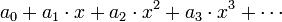
\includegraphics[scale=.6]{graphics/c0f960b20df765fdc843e8c076225d5e.png}
% \caption{a\_0 + a\_1 \textbackslash{}cdot x + a\_2 \textbackslash{}cdot
% x\^{}2 + a\_3 \textbackslash{}cdot x\^{}3 + \textbackslash{}cdots}
\end{figure}

The \emph{a\textsubscript{i}} are called the \emph{coefficients} of the
series. Such sums can be added, multiplied etc., where the new
coefficients of the powers of \emph{x} are calculated according to the
usual rules.

If one is not interested in evaluating such a series for particular
values of \emph{x}, or in other words, if convergence doesn't play a
role, then such a collection of coefficients is called \emph{formal
power series}. It can be treated like a new kind of number.

\textbf{Task}: Implement formal power series as a numeric type.
Operations should at least include \emph{addition},
\emph{multiplication}, \emph{division} and additionally non-numeric
operations like \emph{differentiation} and \emph{integration} (with an
integration constant of zero). Take care that your implementation deals
with the potentially infinite number of coefficients.

As an example, define the power series of sine and cosine in terms of
each other using integration, as in

\begin{figure}[htbp]
\centering
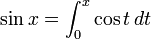
\includegraphics[scale=.6]{graphics/57270a0aaa24e849c7139b71fc5a2879.png}
% \caption{\textbackslash{}sin x = \textbackslash{}int\_0\^{}x
% \textbackslash{}cos t\textbackslash{}, dt}
\end{figure}

\begin{figure}[htbp]
\centering
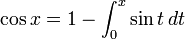
\includegraphics[scale=.6]{graphics/a9aea137ca2037a12d1cf6b4db76aa23.png}
% \caption{\textbackslash{}cos x = 1 - \textbackslash{}int\_0\^{}x
% \textbackslash{}sin t\textbackslash{}, dt}
\end{figure}

\textbf{Goals}: Demonstrate how the language handles new numeric types
and delayed (or \emph{lazy}) evaluation.

\begin{wideverbatim}

With a 'lazy' function, as a frontend to
'[http://software-lab.de/doc/refC.html#cache cache]',

(de lazy Args
   (def (car Args)
      (list (cadr Args)
         (cons 'cache (lit (cons))
            (list 'pack (list 'char (list 'hash (caadr Args))) (caadr Args))
            (cddr Args) ) ) ) )

we can build a formal power series functionality:

(scl 20)

(de fpsOne (N)
   (if (=0 N) 1.0 0) )

(de fpsInverse (N X)
   (last
      (make
         (let Res1 (- (link (*/ 1.0 1.0 (X 0))))
            (for I N
               (link
                  (*/
                     (sum '((Res J) (*/ (X J) Res 1.0))
                        (made)
                        (range I 1) )
                     Res1
                     1.0 ) ) ) ) ) ) )

(de fpsAdd (N X Y)
   (+ (X N) (Y N)) )

(de fpsSub (N X Y)
   (- (X N) (Y N)) )

(de fpsMul (N X Y)
   (sum
      '((I)
         (*/ (X I) (Y (- N I)) 1.0) )
      (range 0 N) ) )

(de fpsDiv (N X Y)
   (sum
      '((I)
         (*/ (X I) (fpsInverse (- N I) Y) 1.0) )
      (range 0 N) ) )

(de fpsDifferentiate (N)
   (curry (X) (N)
      (* (X (inc N)) N) ) )

\end{wideverbatim}

\begin{wideverbatim}

(de fpsIntegrate (X)
   (curry (X) (N)
      (or
         (=0 N)
         (*/ (X (dec N)) N) ) ) )

(lazy fpsSin (N)
   ((fpsIntegrate fpsCos) N) )

(lazy fpsCos (N)
   (fpsSub N fpsOne (fpsIntegrate fpsSin)) )

(lazy fpsTan (N)
   (fpsDiv N fpsSin fpsCos) )

(lazy fpsExp (N)
   (if (=0 N)
      1.0
      ((fpsIntegrate fpsExp) N) ) )


Test:

(prin "SIN:")
(for N (range 1 11 2)
   (prin " " (round (fpsSin N) 9)) )
(prinl)

(prin "COS:")
(for N (range 0 10 2)
   (prin " " (round (fpsCos N) 9)) )
(prinl)

(prin "TAN:")
(for N (range 1 13 2)
   (prin " " (round (fpsTan N) 7)) )
(prinl)

(prin "EXP:")
(for N (range 0 6)
   (prin " " (round (fpsExp N) 7)) )
(prinl)

Output:

SIN: 1.000000000 -0.166666667 0.008333333 -0.000198413 0.000002756 -0.000000025
COS: 1.000000000 -0.500000000 0.041666667 -0.001388889 0.000024802 -0.000000276
TAN: 1.0000000 0.3333333 0.1333333 0.0539683 0.0218695 0.0088632 0.0035921
EXP: 1.0000000 1.0000000 0.5000000 0.1666667 0.0416667 0.0083333 0.0013889

\end{wideverbatim}

\pagebreak{}
\section*{Formatted numeric output}

Express a number in decimal as a fixed-length string with leading zeros.

For example, the number 7.125 could be expressed as ``00007.125''.

\begin{wideverbatim}

(pad 9 (format 7125 3))
(pad 9 (format 7125 3 ","))  # European format

\end{wideverbatim}

\pagebreak{}
\section*{Forward difference}

Provide code that produces a list of numbers which is the n-th order
forward difference, given a non-negative integer (specifying the order)
and a list of numbers. The first-order forward difference of a list of
numbers (A) is a new list (B) where B\textsubscript{n} =
A\textsubscript{n+1} - A\textsubscript{n}. List B should have one less
element as a result. The second-order forward difference of A will be
the same as the first-order forward difference of B. That new list will
have two fewer elements than A and one less than B. The goal of this
task is to repeat this process up to the desired order.

For a more formal description, see the related
\href{http://mathworld.wolfram.com/ForwardDifference.html}{Mathworld
article}.

Algorithmic options:

\begin{itemize}
\item
  Iterate through all previous forward differences and re-calculate a
  new array each time.
\item
  Use this formula (from
  \href{http://en.wikipedia.org/wiki/Forward\_difference}{Wikipedia}):
\end{itemize}

\begin{figure}[H]
\centering
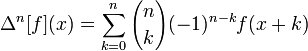
\includegraphics[scale=.6]{graphics/53bd5a42fe34b643a67c4232e71e3f99.png}
% \caption{\textbackslash{}Delta\^{}n {[}f{]}(x)=
% \textbackslash{}sum\_\{k=0\}\^{}n \{n \textbackslash{}choose k\}
% (-1)\^{}\{n-k\} f(x+k)}
\end{figure}

(\emph{Pascal's Triangle} may be useful for this option)



\begin{wideverbatim}

(de fdiff (Lst)
   (mapcar - (cdr Lst) Lst) )

(for (L (90 47 58 29 22 32 55 5 55 73) L (fdiff L))
   (println L) )

Output:

(90 47 58 29 22 32 55 5 55 73)
(-43 11 -29 -7 10 23 -50 50 18)
(54 -40 22 17 13 -73 100 -32)
(-94 62 -5 -4 -86 173 -132)
(156 -67 1 -82 259 -305)
(-223 68 -83 341 -564)
(291 -151 424 -905)
(-442 575 -1329)
(1017 -1904)
(-2921)

\end{wideverbatim}

\pagebreak{}
\section*{Four bit adder}

The aim of this task is to "\emph{simulate}" a four-bit adder ``chip''.
This ``chip'' can be realized using four
\href{http://en.wikipedia.org/wiki/Adder\_(electronics)\#Full\_adder}{1-bit
full adders}. Each of these 1-bit full adders can be with two
\href{http://en.wikipedia.org/wiki/Adder\_(electronics)\#Half\_adder}{half
adders} and an \emph{or}
\href{http://en.wikipedia.org/wiki/Logic\_gate}{gate}. Finally a half
adder can be made using a \emph{xor} gate and an \emph{and} gate. The
\emph{xor} gate can be made using two \emph{not}s, two \emph{and}s and
one \emph{or}.

\textbf{Not}, \textbf{or} and \textbf{and}, the only allowed ``gates''
for the task, can be ``imitated'' by using the \emph{bitwise
  operators} of your language. If there is not a \emph{bit type} in
your language, to be sure that the \emph{not} does not ``invert'' all
the other bits of the basic type (e.g. a byte) we are not interested
in, you can use an extra \emph{nand} (\emph{and} then \emph{not}) with
the constant 1 on one input.

Instead of optimizing and reducing the number of gates used for the
final 4-bit adder, build it in the most straightforward way,
\emph{connecting} the other ``constructive blocks'', in turn made of
``simpler'' and ``smaller'' ones.

\ctable[caption = {Schematics of the ``constructive blocks'' },
pos = H, center, botcap]{llll}
{% notes
}
{% rows
\FL
Xor gate done with \\ ands, ors and nots & A half adder & A full adder & A
4-bit adder
\ML
{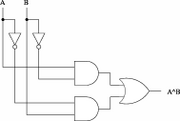
\includegraphics[scale=.6]{graphics/180px-Xor.png}} & {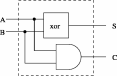
\includegraphics[scale=.6]{graphics/Halfadder.png}} & {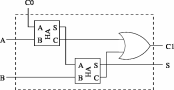
\includegraphics[scale=.6]{graphics/Fulladder.png}} & {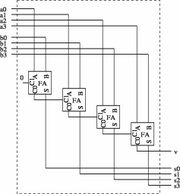
\includegraphics[scale=.6]{graphics/180px-4bitsadder.png}}
\LL
}

Solutions should try to be as descriptive as possible, making it as easy
as possible to identify ``connections'' between higher-order ``blocks''.
It is not mandatory to replicate the syntax of higher-order blocks in
the atomic ``gate'' blocks, i.e. basic ``gate'' operations can be
performed as usual bitwise operations, or they can be ``wrapped'' in a
\emph{block} in order to expose the same syntax of higher-order blocks,
at implementers' choice.

To test the implementation, show the sum of two four-bit numbers (in
binary).

\begin{wideverbatim}

(de halfAdder (A B)  #> (Carry . Sum)
   (cons
      (and A B)
      (xor A B) ) )

(de fullAdder (A B C)  #> (Carry . Sum)
   (let (Ha1 (halfAdder C A)  Ha2 (halfAdder (cdr Ha1) B))
      (cons
         (or (car Ha1) (car Ha2))
         (cdr Ha2) ) ) )

(de 4bitsAdder (A4 A3 A2 A1  B4 B3 B2 B1)  #> (V S4 S3 S2 S1)
   (let
      (Fa1 (fullAdder A1 B1)
         Fa2 (fullAdder A2 B2 (car Fa1))
         Fa3 (fullAdder A3 B3 (car Fa2))
         Fa4 (fullAdder A4 B4 (car Fa3)) )
      (list
         (car Fa4)
         (cdr Fa4)
         (cdr Fa3)
         (cdr Fa2)
         (cdr Fa1) ) ) )

Output:

: (4bitsAdder NIL NIL NIL T  NIL NIL NIL T)
-> (NIL NIL NIL T NIL)

: (4bitsAdder NIL T NIL NIL  NIL NIL T T)
-> (NIL NIL T T T)

: (4bitsAdder NIL T T T  NIL T T T)
-> (NIL T T T NIL)

: (4bitsAdder T T T T  NIL NIL NIL T)
-> (T NIL NIL NIL NIL)

\end{wideverbatim}

\pagebreak{}
\section*{Fractal tree}

Generate and draw a fractal tree.

To draw a fractal tree is simple:

\begin{enumerate}
\item
  Draw the trunk
\item
  At the end of the trunk, split by some angle and draw two branches
\item
  Repeat at the end of each branch until a sufficient level of branching
  is reached
\end{enumerate}

\begin{wideverbatim}

This uses the 'brez' line drawing function from
[[Bitmap/Bresenham's line algorithm#PicoLisp]].

(load "@lib/math.l")

(de fractalTree (Img X Y A D)
   (unless (=0 D)
      (let (R (*/ A pi 180.0)  DX (*/ (cos R) D 0.2)  DY (*/ (sin R) D 0.2))
         (brez Img X Y DX DY)
         (fractalTree Img (+ X DX) (+ Y DY) (+ A 30.0) (dec D))
         (fractalTree Img (+ X DX) (+ Y DY) (- A 30.0) (dec D)) ) ) )

(let Img (make (do 300 (link (need 400 0))))       # Create image 400 x 300
   (fractalTree Img 200 300 -90.0 10)              # Draw tree
   (out "img.pbm"                                  # Write to bitmap file
      (prinl "P1")
      (prinl 400 " " 300)
      (mapc prinl Img) ) )

\end{wideverbatim}

\pagebreak{}
\section*{Function composition}

Create a function, compose, whose two arguments \emph{f} and \emph{g},
are both functions with one argument. The result of compose is to be a
function of one argument, (lets call the argument \emph{x}), which works
like applying function \emph{f} to the result of applying function
\emph{g} to \emph{x}, i.e,

compose(\emph{f}, \emph{g}) (\emph{x}) = \emph{f}(\emph{g}(\emph{x}))

Reference:
\href{http://en.wikipedia.org/wiki/Function\_composition\_(computer\_science)}{Function
composition}

Hint: In some languages, implementing compose correctly requires
creating a
\href{http://en.wikipedia.org/wiki/Closure\_(computer\_science)}{closure}.


\begin{wideverbatim}

(de compose (F G)
   (curry (F G) (X)
      (F (G X)) ) )

(def 'a (compose inc dec))
(def 'b (compose 'inc 'dec))
(def 'c (compose '((A) (inc A)) '((B) (dec B))))

: (a 7)
-> 7

: (b 7)
-> 7

: (c 7)
-> 7

\end{wideverbatim}

\pagebreak{}
\section*{Function definition}

A function is a body of code that returns a value. The value returned
may depend on arguments provided to the function.

Write a definition of a function called ``multiply'' that takes two
arguments and returns their product. (Argument types should be chosen so
as not to distract from showing how functions are created and values
returned).

\begin{wideverbatim}

(de multiply (A B)
   (* A B) )

\end{wideverbatim}

\pagebreak{}
\section*{Function frequency}

Display - for a program or runtime environment (whatever suites the
style of your language) - the top ten most frequently occurring
functions (or also identifiers or tokens, if preferred).

This is a static analysis: The question is not how often each function
is actually executed at runtime, but how often it is used by the
programmer.

Besides its practical usefulness, the intent of this task is to show how
to do self-inspection within the language.


\begin{wideverbatim}

(let Freq NIL
   (for "L" (filter pair (extract getd (all)))
      (for "F"
         (filter atom
            (fish '((X) (or (circ? X) (getd X)))
               "L" ) )
         (accu 'Freq "F" 1) ) )
   (for X (head 10 (flip (by cdr sort Freq)))
      (tab (-7 4) (car X) (cdr X)) ) )

Output, for the system in debug mode plus the above code:

quote   310
car     236
cdr     181
setq    148
let     136
if      127
and     124
cons    110
cadr     80
or       76

If the condition in the 5th line (getd X) is replaced with (sym? X), then all
symbols are counted, and the output is

X       566
quote   310
car     236
cdr     181
C       160
N       157
L       155
Lst     152
setq    148
T       144

And if it is replaced with (num? X), it is

1        71
0        38
2        27
3        17
7         9
-1        9
100       8
48        6
43        6
12        6

\end{wideverbatim}



% %%%%%%%%%%%%%%%%%%%%%%%% referenc.tex %%%%%%%%%%%%%%%%%%%%%%%%%%%%%%
% sample references
% %
% Use this file as a template for your own input.
%
%%%%%%%%%%%%%%%%%%%%%%%% Springer-Verlag %%%%%%%%%%%%%%%%%%%%%%%%%%
%
% BibTeX users please use
% \bibliographystyle{}
% \bibliography{}
%
\biblstarthook{In view of the parallel print and (chapter-wise) online publication of your book at \url{www.springerlink.com} it has been decided that -- as a genreral rule --  references should be sorted chapter-wise and placed at the end of the individual chapters. However, upon agreement with your contact at Springer you may list your references in a single seperate chapter at the end of your book. Deactivate the class option \texttt{sectrefs} and the \texttt{thebibliography} environment will be put out as a chapter of its own.\\\indent
References may be \textit{cited} in the text either by number (preferred) or by author/year.\footnote{Make sure that all references from the list are cited in the text. Those not cited should be moved to a separate \textit{Further Reading} section or chapter.} The reference list should ideally be \textit{sorted} in alphabetical order -- even if reference numbers are used for the their citation in the text. If there are several works by the same author, the following order should be used: 
\begin{enumerate}
\item all works by the author alone, ordered chronologically by year of publication
\item all works by the author with a coauthor, ordered alphabetically by coauthor
\item all works by the author with several coauthors, ordered chronologically by year of publication.
\end{enumerate}
The \textit{styling} of references\footnote{Always use the standard abbreviation of a journal's name according to the ISSN \textit{List of Title Word Abbreviations}, see \url{http://www.issn.org/en/node/344}} depends on the subject of your book:
\begin{itemize}
\item The \textit{two} recommended styles for references in books on \textit{mathematical, physical, statistical and computer sciences} are depicted in ~\cite{science-contrib, science-online, science-mono, science-journal, science-DOI} and ~\cite{phys-online, phys-mono, phys-journal, phys-DOI, phys-contrib}.
\item Examples of the most commonly used reference style in books on \textit{Psychology, Social Sciences} are~\cite{psysoc-mono, psysoc-online,psysoc-journal, psysoc-contrib, psysoc-DOI}.
\item Examples for references in books on \textit{Humanities, Linguistics, Philosophy} are~\cite{humlinphil-journal, humlinphil-contrib, humlinphil-mono, humlinphil-online, humlinphil-DOI}.
\item Examples of the basic Springer style used in publications on a wide range of subjects such as \textit{Computer Science, Economics, Engineering, Geosciences, Life Sciences, Medicine, Biomedicine} are ~\cite{basic-contrib, basic-online, basic-journal, basic-DOI, basic-mono}. 
\end{itemize}
}

\begin{thebibliography}{99.}%
% and use \bibitem to create references.
%
% Use the following syntax and markup for your references if 
% the subject of your book is from the field 
% "Mathematics, Physics, Statistics, Computer Science"
%
% Contribution 
\bibitem{science-contrib} Broy, M.: Software engineering --- from auxiliary to key technologies. In: Broy, M., Dener, E. (eds.) Software Pioneers, pp. 10-13. Springer, Heidelberg (2002)
%
% Online Document
\bibitem{science-online} Dod, J.: Effective substances. In: The Dictionary of Substances and Their Effects. Royal Society of Chemistry (1999) Available via DIALOG. \\
\url{http://www.rsc.org/dose/title of subordinate document. Cited 15 Jan 1999}
%
% Monograph
\bibitem{science-mono} Geddes, K.O., Czapor, S.R., Labahn, G.: Algorithms for Computer Algebra. Kluwer, Boston (1992) 
%
% Journal article
\bibitem{science-journal} Hamburger, C.: Quasimonotonicity, regularity and duality for nonlinear systems of partial differential equations. Ann. Mat. Pura. Appl. \textbf{169}, 321--354 (1995)
%
% Journal article by DOI
\bibitem{science-DOI} Slifka, M.K., Whitton, J.L.: Clinical implications of dysregulated cytokine production. J. Mol. Med. (2000) doi: 10.1007/s001090000086 
%
\bigskip

% Use the following (APS) syntax and markup for your references if 
% the subject of your book is from the field 
% "Mathematics, Physics, Statistics, Computer Science"
%
% Online Document
\bibitem{phys-online} J. Dod, in \textit{The Dictionary of Substances and Their Effects}, Royal Society of Chemistry. (Available via DIALOG, 1999), 
\url{http://www.rsc.org/dose/title of subordinate document. Cited 15 Jan 1999}
%
% Monograph
\bibitem{phys-mono} H. Ibach, H. L\"uth, \textit{Solid-State Physics}, 2nd edn. (Springer, New York, 1996), pp. 45-56 
%
% Journal article
\bibitem{phys-journal} S. Preuss, A. Demchuk Jr., M. Stuke, Appl. Phys. A \textbf{61}
%
% Journal article by DOI
\bibitem{phys-DOI} M.K. Slifka, J.L. Whitton, J. Mol. Med., doi: 10.1007/s001090000086
%
% Contribution 
\bibitem{phys-contrib} S.E. Smith, in \textit{Neuromuscular Junction}, ed. by E. Zaimis. Handbook of Experimental Pharmacology, vol 42 (Springer, Heidelberg, 1976), p. 593
%
\bigskip
%
% Use the following syntax and markup for your references if 
% the subject of your book is from the field 
% "Psychology, Social Sciences"
%
%
% Monograph
\bibitem{psysoc-mono} Calfee, R.~C., \& Valencia, R.~R. (1991). \textit{APA guide to preparing manuscripts for journal publication.} Washington, DC: American Psychological Association.
%
% Online Document
\bibitem{psysoc-online} Dod, J. (1999). Effective substances. In: The dictionary of substances and their effects. Royal Society of Chemistry. Available via DIALOG. \\
\url{http://www.rsc.org/dose/Effective substances.} Cited 15 Jan 1999.
%
% Journal article
\bibitem{psysoc-journal} Harris, M., Karper, E., Stacks, G., Hoffman, D., DeNiro, R., Cruz, P., et al. (2001). Writing labs and the Hollywood connection. \textit{J Film} Writing, 44(3), 213--245.
%
% Contribution 
\bibitem{psysoc-contrib} O'Neil, J.~M., \& Egan, J. (1992). Men's and women's gender role journeys: Metaphor for healing, transition, and transformation. In B.~R. Wainrig (Ed.), \textit{Gender issues across the life cycle} (pp. 107--123). New York: Springer.
%
% Journal article by DOI
\bibitem{psysoc-DOI}Kreger, M., Brindis, C.D., Manuel, D.M., Sassoubre, L. (2007). Lessons learned in systems change initiatives: benchmarks and indicators. \textit{American Journal of Community Psychology}, doi: 10.1007/s10464-007-9108-14.
%
%
% Use the following syntax and markup for your references if 
% the subject of your book is from the field 
% "Humanities, Linguistics, Philosophy"
%
\bigskip
%
% Journal article
\bibitem{humlinphil-journal} Alber John, Daniel C. O'Connell, and Sabine Kowal. 2002. Personal perspective in TV interviews. \textit{Pragmatics} 12:257--271
%
% Contribution 
\bibitem{humlinphil-contrib} Cameron, Deborah. 1997. Theoretical debates in feminist linguistics: Questions of sex and gender. In \textit{Gender and discourse}, ed. Ruth Wodak, 99--119. London: Sage Publications.
%
% Monograph
\bibitem{humlinphil-mono} Cameron, Deborah. 1985. \textit{Feminism and linguistic theory.} New York: St. Martin's Press.
%
% Online Document
\bibitem{humlinphil-online} Dod, Jake. 1999. Effective substances. In: The dictionary of substances and their effects. Royal Society of Chemistry. Available via DIALOG. \\
http://www.rsc.org/dose/title of subordinate document. Cited 15 Jan 1999
%
% Journal article by DOI
\bibitem{humlinphil-DOI} Suleiman, Camelia, Daniel C. O�Connell, and Sabine Kowal. 2002. `If you and I, if we, in this later day, lose that sacred fire...�': Perspective in political interviews. \textit{Journal of Psycholinguistic Research}. doi: 10.1023/A:1015592129296.
%
%
%
\bigskip
%
%
% Use the following syntax and markup for your references if 
% the subject of your book is from the field 
% "Computer Science, Economics, Engineering, Geosciences, Life Sciences"
%
%
% Contribution 
\bibitem{basic-contrib} Brown B, Aaron M (2001) The politics of nature. In: Smith J (ed) The rise of modern genomics, 3rd edn. Wiley, New York 
%
% Online Document
\bibitem{basic-online} Dod J (1999) Effective Substances. In: The dictionary of substances and their effects. Royal Society of Chemistry. Available via DIALOG. \\
\url{http://www.rsc.org/dose/title of subordinate document. Cited 15 Jan 1999}
%
% Journal article by DOI
\bibitem{basic-DOI} Slifka MK, Whitton JL (2000) Clinical implications of dysregulated cytokine production. J Mol Med, doi: 10.1007/s001090000086
%
% Journal article
\bibitem{basic-journal} Smith J, Jones M Jr, Houghton L et al (1999) Future of health insurance. N Engl J Med 965:325--329
%
% Monograph
\bibitem{basic-mono} South J, Blass B (2001) The future of modern genomics. Blackwell, London 
%
\end{thebibliography}

